\chapter{Results and Discussion}

% Chapter giving an overview of the numerical results obtained from the implementation

All simulations were carried out on the standard Pitz-Daily backward facing step geometry provided with OpenFOAM. The kinematic viscosity of $\nu=10^{-5}\,\mathrm{m}^2/\mathrm{s}$ and the inlet velocity of $u=10\,\mathrm{m}/\mathrm{s}$ were kept constant for all runs. Using this inlet velocity and the channel width $L=50.8\,\mathrm{mm}$, the Reynolds number of the flow can be approximated as: $$ Re=\frac{uL}{\nu}=50800$$

In order to provide a somewhat objective measure of comparison between the results of the method using different sets of parameters, a vertical line profile of the mean magnitude of the unfiltered velocity field was taken at the location shown in Fig. \ref{fig:line_location} after each run. As well, a simulation using a simple direct solution of the Navier-Stokes equations was performed as a baseline. It must be noted that this is not a true DNS comparison, as the simulation was performed on the same grid as used for all of the following TLES testing, and so is not fine enough to resolve the full range of scales of the system in general. Since such a fully-resolved DNS simulation was prohibitively time-consuming for this project, the under-resolved baseline case was considered acceptable to at least check for any large deviations resulting from the methods being tested, and for simplicity is referred to as DNS in the following analysis. The location of the line was chosen to be at the minimum value of the recirculation vortex in the DNS baseline, so as to have a distinct feature to compare with between runs.

\begin{figure}[!b]
\centering
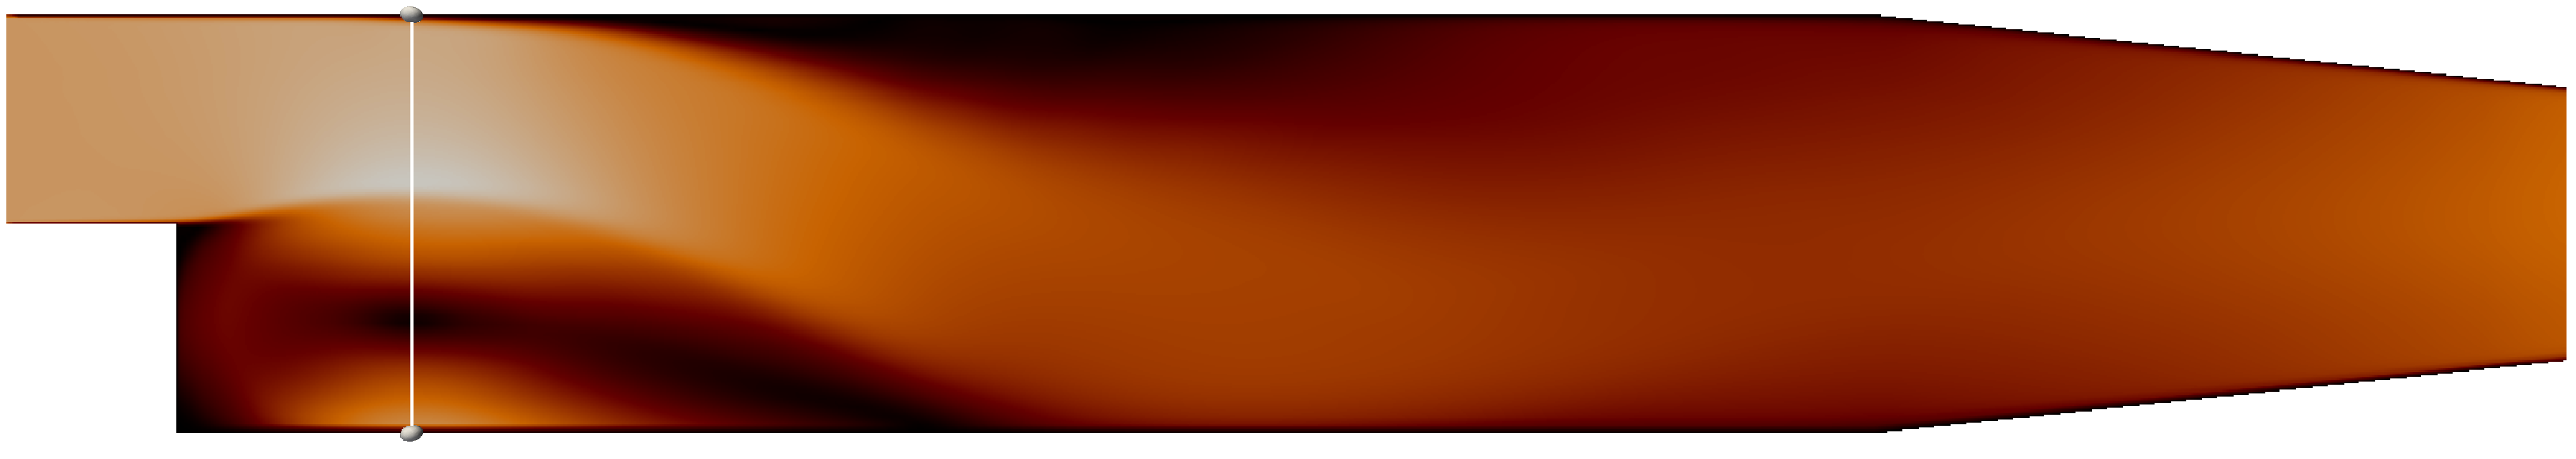
\includegraphics[width=0.75\textwidth]{figures/line_location.pdf}
\caption{Representative image of a $|\bar{u}|_{\mathrm{mean}}$ velocity field with a white line showing the location $x=28.6\,\mathrm{mm}$ past the step at which the comparison profiles were captured}
\label{fig:line_location}
\end{figure}

To start with, several simulations were run using only the basic TLES implementation, with no regularization or DC. This gave one free parameter to be varied, the filter width ratio $r$, and the resulting profiles were taken at an end time of $t_\mathrm{final}=0.1$ using a time step of $\Delta t=10^{-6}$ for all runs. It was observed that the simulation becomes unstable if the filter width is made too large, and so this time step was chosen as it gave a small range of values, up to $r\approx 28$, for which the base method was stable and any effects of varying $r$ in isolation could be observed.

The results of this initial study are shown in Fig. \ref{fig:line_data_no_reg} and the profiles from the various runs are seen to lie almost completely atop one another. This would seem to suggest that the effect of $r$ is minimal within the range of values which are stable without regularization.

\begin{figure}[!htb]
\centering
\includegraphics[width=0.75\textwidth]{figures/line_data_no_reg.pdf}
\caption{Comparison of line profiles from the $|\bar{u}|_{\mathrm{mean}}$ velocity field at $x=28.6\,\mathrm{mm}$ for various values of filter width $r$, taken at $t_\mathrm{final}=0.1$ using $\Delta t=10^{-6}$}
\label{fig:line_data_no_reg}
\end{figure}

\section{Divergence Cleaning}

The effects of adding DC to the method as per the projection method outlined in section \ref{sec:DC} were investigated next. A small increase in the stable range of the filter width $r$ was observed, with the largest stable value for $r$ increasing from $r=4.4$ to $r=4.7$ when $\Delta t=10^{-5}$, and from $r=28$ to $r=29$ for a $\Delta t=10^{-6}$ time step. Simulations were run with DC included in the simulations for the same already stable values of $r$ as in the previous set as well as for the now stabilized $r=29$ case, and the results are shown in Fig. \ref{fig:line_data_DC}. This allowed for potential comparison between the effects of DC both when it was and was not required to achieve stability in the first instance.

Unlike with the base TLES simulations, all of the runs with DC are seen to be no longer as perfectly concident with the baseline simulation, although the deviation is relatively minor and the variations of $r$ still appear to have little discernible impact on the results. Additionally, the runtime of the simulations increased by only between 5-11\% for the values of $r$ with a counterpart simulation not using DC, indicating decent efficiency of the DC implementation using an iterative solver with a relaxed tolerance, as discussed in section \ref{sec:DC} and chapter \ref{chap:Imp}. Since DC was only able to provide stabilization over a small range of additional filter widths, this would suggest both that non-zero divergence is indeed present in the simulations, since DC did have an effect, but also that it is not itself the cause of the instability, since then DC would have been expected to provide a much greater degree of stabilization. It is therefore posited that the stabilizing effects of DC are possibly due simply to reducing the overall velocity magnitude when removing the non-physical component, which for instabilities whose growth rates were but slightly greater than one was enough to bring them back inside the stable region.

\begin{figure}[!tb]
\centering
\includegraphics[width=0.75\textwidth]{figures/line_data_DC.pdf}
\caption{Comparison of line profiles from the $|\bar{u}|_{\mathrm{mean}}$ velocity field at $x=28.6\,\mathrm{mm}$ for various values of filter width $r$ with divergence cleaning, taken at $t_\mathrm{final}=0.1$ using $\Delta t=10^{-6}$}
\label{fig:line_data_DC}
\end{figure}

\section{Regularization}

In Fig. \ref{fig:line_data_reg} is shown the result of a run at $r=30$, using regularization with a control value of $\chi=32000$ to stabilize the simulation. This value of $\chi$ was chosen so as to be slightly larger than the minimal value for which the simulation was found to be stable for $r=30$, as discussed later in this chapter. It is observed that while the shape of the profile is very similar to the baseline case, the data shown was collected only after propogating the simulation through 87X as many timesteps, to a $t_\mathrm{final}=8.4$ compared to $0.1$ for the baseline (and all other profiles shown.) The final time for comparison was chosen to be the time when the minimum of the recirculation vortex in the regularized run reached the same location as in the compared against baseline profile. Such good agreement between the profiles when matching such a recognizable feature as the vortex minimum suggests that the regularization stabilized simulation seems to evolve through the same sequence as without regularization, only at a \emph{much} slower rate.

\begin{figure}[!htb]
\centering
\includegraphics[width=0.75\textwidth]{figures/line_data_reg.pdf}
\caption{Line profile from the $|\bar{u}|_{\mathrm{mean}}$ velocity field at $x=28.6\,\mathrm{mm}$ for $r=30$ with regularization. $\chi = 32000$, $\tilde{r}=100$, $\Delta t=10^{-6}$, $t_\mathrm{final}=0.1$ for DNS and $t_\mathrm{final}=8.4$ for $r=30$}
\label{fig:line_data_reg}
\end{figure}

Two slight modifications of the regularization term in Eq. (\ref{eq:reg}) were also briefly investigated. The first used the de-convoluted velocity in place of the filtered velocity as $-\chi(u-\tilde{u})$ but it was found to provide less of a stabilizing influence. In particular, making $\chi$ too large caused the simulation to again become unstable, meaning there was a limited range of acceptable $\chi$ which which provided stability, while when using the filtered velocity no such upper bound was encountered during testing. As well, this range of acceptable $\chi$ values contracted with increasing filter widths, eventually vanishing entirely for large enough $r$, a limitation that was also not encountered for the formulation of Eq. (\ref{eq:reg}), which was able to stabilize all tested values of $r$ simply through comensurate increase in $\chi$.

The second modification changed the computation of $\tilde{u}$. Instead of filtering the de-convoluted value, the filtered value $\bar{u}$ was simply filtered again with the same condition $\tilde{T}>T$ on the filter width of the second filtering operation, in effect producing a regulariztion term $-\chi(\bar{u}-\tilde{\bar{u}})$. This set-up followed more closely the methodology of \AA kervik et al. \cite{Akervik2006}, but was not investigated very deeply due to time constraints, and as it was found to produce almost exactly the same results as Eq. (\ref{eq:reg}), no immediate benefits were obvious.

\subsection{Minimum Stabilizing $\chi$}

Since most cases of instability in the simulation manifested within the first few dozen time steps (approx. 30-40 or less), and given the large number of parameter sets that required testing, for the purposes of the following section a simulation was considered `stable' if it ran for at least 100 timesteps without failing. It is noted that a small number of the runs performed crashed even after 80+ timesteps, so this 100 timestep rule is certainly not an ironclad guarantee of stability over a much longer run. However, as in all of these cases it was the point of transition from unstable to stable that was under investigation, it suffices to warn that the reported minimal $\chi$ values required for stability should be regarded as providing only marginal stability, and slightly larger values might be safer in real simulations to provide some margin of safety.

To investigate any potential relationship between the smallest value of $\chi$ for which a given set-up was stable and the other simulation parameters ($r$, $\tilde{r}$, and $\Delta t$) three series of simulations were run where $r$ was varied while maintaining $\tilde{r}$ and $\Delta t$ constant. Results from the first of these series is found in Fig. \ref{fig:min_chi_dt5_r100} for $\Delta t=10^{-5}$ and $\tilde{r}=100$. A clear linear relation is observed between $\chi_{\mathrm{min}}$ and $r$, with the trendline and equation of the linear least squares regression also shown on the chart, along with the $R^2$ measure of the goodness of fit (in this case an excellently high $0.9998$.) The value of the regression slope is quite large, at just over $21000$, indicative of a high degree of regularization required to achieve stability for large filter widths and underscoring the reason for the slow time evolution of the stabilized systems, as \AA kervik et al. \cite{Akervik2006} clearly demonstrate that large values of $\chi$ will greatly reduce the convergence rate of the system towards its steady state.

\begin{figure}[!tb]
\centering
\includegraphics[width=0.75\textwidth]{figures/min_chi_dt5_r100.pdf}
\caption{Minimum $\chi$ values required to stabilize simulation for various values of $r$, using $\Delta t=10^{-5}$ and $\tilde{r}=100$, and showing the linear least squares regression}
\label{fig:min_chi_dt5_r100}
\end{figure}

Fig. \ref{fig:min_chi_dt5_r10} shows the second series of data  with the time step still at $\Delta t=10^{-5}$ but reducing the regularization filter width ratio to $\tilde{r}=10$. An extremely linear relation is observed, with only a slight increase in the slope and slight decrease in the intercept, and both changes being less than $2.5\%$ compared to the order of magnitude decrease in $\tilde{r}$. This suggests only a weak relation between the required $\chi$ and $\tilde{r}$ but would ccertainly require more data points to confirm, particularly for values of $\tilde{r}$ which are very large and those close to the base TLES filter width where $\tilde{r}$ approaches one.

\begin{figure}[!tb]
\centering
\includegraphics[width=0.75\textwidth]{figures/min_chi_dt5_r10.pdf}
\caption{Minimum $\chi$ values required to stabilize simulation for various values of $r$, using $\Delta t=10^{-5}$ and $\tilde{r}=10$, and showing the linear least squares regression}
\label{fig:min_chi_dt5_r10}
\end{figure}

Data for the third and final series can be found in Fig. \ref{fig:min_chi_dt6_r100}, this time returning the regularization filter width ratio to $\tilde{r}=100$ but now decreasing the time step to $\Delta t=10^{-6}$. Once again the trend is linear, with the slope for this case being somewhat lower at $19377$, but still only a decrease of $8.4\%$  compared to an order of magnitude decrease in the time step, suggesting that the slope has only a weak dependence on the time step similarly as on $\tilde{r}$. On the other hand, the intercept displays a much stronger dependence on change in $\Delta t$, decreasing almost exactly sixfold, but additional data points would again be necessary to try and quantify the exact nature of the dependence relation.

\begin{figure}[!t]
\centering
\includegraphics[width=0.75\textwidth]{figures/min_chi_dt6_r100.pdf}
\caption{Minimum $\chi$ values required to stabilize simulation for various values of $r$, using $\Delta t=10^{-6}$ and $\tilde{r}=100$, and showing the linear least squares regression}
\label{fig:min_chi_dt6_r100}
\end{figure}

It was observed that when analyzing the data output step-by-step for an unstable simulation, the problematic growth is observed to occur precisely at the sharp corner of the backwards facing step in the geometry. Such an obvious focal point would suggest a likely strong dependence of the stability behaviour for the TLES solver on the specific geometry under consideration. As such, any functional relationship between $\chi_{mathrm{min}}$ and the other method parameters would most likely be valid only for the geometry (and probably also the specific mesh) on which the data was measured.

As well, the initial conditions used to initialize the simulation can also play a large role. While not thoroughly investigated by any means, it was found that using the data from the end of the baseline simulation for the starting values of a new simulation allowed extremely large filter widths to be used stably without regularization. For a time step of $\Delta t=10^{-6}$, filter width ratios of over $r=1200$ were able to run through 100 steps without failing compared to a maximum of $r=28$ with a uniform zero initial velocity condition, although a test at $r=1400$ still crashed so it is certainly not a complete cure for the instability. And while using such a well-developed baseline as a starting condition would be expensive in general (and rather defeat the purpose of an LES based model), since most runs failed within only a few dozen time steps or else not at all, it could be fruitful to investigate whether even just a few tens of interations at the start of a run with a stable parameter set could be used to greatly increase the stability of a full simulation with a more desirable but less stable model configuration.

Finally, while the investigation focused on achieving stabilization when increasing the filter width, it was also observed that a simulation using a time step of $\Delta t=10^{-4}$, which was not stable for any filter width under the base method, was also able to be stabilized with a large enough $\chi$. This could offer one potential avenue to mitigate some of the effects of the slower evolution of the regularized system by allowing the use of larger time steps, although further investigation would again be necessary to determine the viability of such an approach.